 Bei Unsupervised Learning haben die Trainings-Daten keine Label. \cite{Sarkar2018} Es ist also kein erwarteter Output bekannt und auch schwer feststellbar ob das Modell korrekte Ergebnisse erzielt. Der Algorithmus bekommt nur die Input-Daten. Er muss anhand dieser Entscheidungen treffen und kategorisieren. \cite{Mueller2016}\newline
	 Das Modell lernt inherente Strukturen, Muster und Beziehungen aus dem Datensatz, ohne dabei Hilfe von außen zu bekommen. \cite{Sarkar2018} Hierbei werden besondere Auffälligkeiten im Datensatz gefunden. \cite{Kirk2014} Die Ergebnisse sind unsicherer als die von Supervised Learning Algorithmen. Sie eignen sich aber, um weitere Informationen zu den Daten zu finden. \cite{Sarkar2018} Deshalb wird diese Art des Machine Learnings oft in explorativen Bereichen eingesetzt, um Daten besser zu verstehen. Unsupervised Learning kann als Vorverarbeitungsschritt des Supervised Learnings eingesetzt werden. Hierbei sollen neue Representatoren für die Daten gefunden werden, um Genauigkeit, Speichernutzung und Geschwindigkeit zu verbessern. \cite{Mueller2016}
	 Unsupervised Learning kann durch verschiedene Methoden angewendet werden: Clusterbildung, Dimensionsreduktion, Anomalie Erkennung und Association rule-mining. \cite{Sarkar2018} Diese werden im Folgenden behandelt.
	 
	 \subsection{Clusterbildung}
	 Ziel der Clusterbildung ist es, dass sich in einem Cluster möglichst ähnliche Daten befinden, die sich zu den Daten außerhalb des Clusters unterscheiden. \cite{Mueller2016} Die Cluster werden durch Muster, Ähnlichkeiten und Verbindungen zwischen den Datensätzen gebildet. \cite{Sarkar2018} Zum Beispiel werden die Elemente in Abbildung \ref{fig:abb3} nach Formen in die Cluster rot, grün und blau eingeordnet. \cite{Sarkar2018}
	  %Die Clusterbildung kann in verschiedene Typen aufgeteilt werden: Centroid based, Hirachical clustering, distribution based und density based. \cite{Sarkar2018}
	 \begin{figure}[h!]
	 	\centering
	 	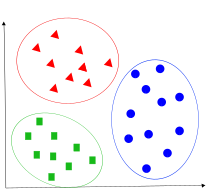
\includegraphics[width=5cm]{Bilder/Cluster.pdf}
	 	\caption{Cluster}
	 	\label{fig:abb3}
	 \end{figure}
	 
	 	\subsubsection{K-Means Algorithmus}
	 	Der K-Means Algorithmus verwendet die Clusterbildung. K steht hierbei für die Anzahl der Cluster, die gebildet werden sollen. \cite{Kirk2014} Es wird versucht, einen Mittelpunkt in jedem Cluster zu finden. Dieser ist der Punkt, der den geringsten Abstand zu allen anderen Punkten in der Region hat. \cite{Mueller2016} Vorteile dieses Algorithmus sind, dass die Cluster sehr genau und kugelförmig sind und der Algorithmus sich einer Lösung annähert. \cite{Kirk2014} \newline
	 	Zu Beginn werden K zufällige Punkte aus dem Datensatz ausgewählt und als Mittelpunkt verwendet. \cite{Kirk2014} Danach werden die verbleibenden Datensätze dem Mittelpunkt mit dem geringsten Abstand zugeordnet und neue Mittelpunkte bestimmt. Diese haben den jeweils geringsten Abstand zu allen anderen Punkten im Cluster. Es werden so lange neue Mittelpunkte bestimmt und Punkte zu neue Clustern zugeordnet, bis es keine Veränderung mehr gibt. \cite{Mueller2016} Der Abstand der Punkte kann mit verschiedenen Methoden berechnet werden. Eine davon ist die Euklidische Distanz, siehe Formel (2). \cite{Kirk2014}
	 	\begin{equation}
	 	d_{euklid}(x,y)= \sqrt{\sum_{i=1}^{n}(x_i - y_i)^2}
	 	\end{equation}
	 	
	 	Im Folgenden wird Beispiel-Code für den Algorithmus erklärt und gezeigt. Hierzu wir die Programmiersprache Python verwendet. Es handelt sich hierbei nur um einen Codeauszug und nicht um ein ganzes Programm.
	 	
	 	\begin{lstlisting}[language=Python]
	 		kmeans = KMeans(n_clusters = 3)
	 		kmeans.fit(X)
	 	\end{lstlisting}
	 	In diesem Abschnitt wird ein K-Means Modell erzeugt und mit Hilfe der Funktion fit trainiert. X enthält die zweidimensionalen Datensätze. Das Modell und die Funktion werden bereits von der scikit-learn Bibliothek bereitgestellt.
	 		\begin{lstlisting}[language=Python]
	 		kmeans.predict(Z)
	 		\end{lstlisting}
	 	Mit predict können nach dem Training den Clustern neue Datensätze Y zugeordnet werden. Die Mittelpunkte und damit auch die Cluster werden dabei nicht mehr verändert. \cite{Mueller2016}
	 	
	 
	 
	 \subsection{Dimensionsreduktion}
	 Die Komplexität des Machine Learning Modells ist abhängig von der Anzahl der Inputs. Sie bestimmen die Zeit- und Speicherkomplexität, sowie die Anzahl der zum Training benötigten Daten. \cite{Alpaydin2004} Dimensionsreduktion wird genutzt um den überladenen Input-Space zu verkleinern. Somit wird die Anzahl der relevanten Features oder Attribute($\widehat{=}$ Dimensionen) für jeden Datensatz reduziert. \cite{Sarkar2018} Wenn die Modelle einfach gehalten werden, sind sie, aufgrund ihrer geringeren Varianz, bei kleinen Datensätzen robuster. \cite{Alpaydin2004} Die Reduktion der Dimensionen erfolgt durch die Auswahl von Hauptfeatures und bedarfsgesteuerten Features. Für diese gibt es zwei Methoden. \cite{Sarkar2018}
	 \newline
	 Für die Feature Extraction werden neue Features, die Kombinationen aus der origninalen Featureliste sind, gesucht. \cite{Alpaydin2004}
	 \newline
	 Bei der Feature Selection werden von d Dimensionen k, mit Hilfe von Subset Selection, ausgewählt. \cite{Alpaydin2004} Die Features, die die meisten Informationen liefern, werden aus der originalen Featureliste ausgewählt, der Rest wird verworfen. Es kommen keine neuen Features hinzu. \cite{Sarkar2018}\newline
	 Ziel der Subset Selection ist es, das beste Subset aus der Featureliste mit einer möglichst geringen Anzahl von Dimensionen und der besten Genauigkeit zu finden. Es gibt $2^{d}$ mögliche Subsets aus denen ausgewählt werden kann. Aufgrund der großen Menge können nicht alle getestet werden, deswegen müssen geeignete Verfahren für die Auswahl genutzt werden. \cite{Alpaydin2004}
	 
	 \subsection{Anomalie Erkennung}
	 Ziel der Anomalie Erkennung ist es, seltene oder laut vorherigen Datensätzen untypische Ereignisse zu erkennen, wie in Abbildung. \ref{fig:abb4} Hier fällt auf, dass ein Wert stark von den Anderen abweicht. \newline
	 Anomalien können auch nach bestimmten Mustern auftreten. In der Trainings-Phase haben alle Input-Daten keine Anomalien, um später Abweichungen von der Norm zu erkennen. Danach kann der Algorithmus zwischen normalen und anomalen Datensätzen unterscheiden. \cite{Sarkar2018}
	 \begin{figure}[h!]
	 	\centering
	 	\includegraphics[width=5cm]{Bilder/Anomalie.pdf}
	 	\caption{Anomalie}
	 	\label{fig:abb4}
	 \end{figure}
	 
	 \subsection{Association rule-mining}
	 Beim Association rule-mining werden Transaktionsdaten untersucht und analysiert, um Muster, sowie mögliche Regeln zu bestimmen. Diese Methode wird auch "market basket analysis" genannt, da sie oft genutzt wird um Einkaufsmuster zu erkennen. \cite{Sarkar2018} \newline
	 In Abbildung \ref{fig:abb5} werden die verschiedenen Formen mit Association rule-mining analysiert. Das Ergebnis ist, dass der Kreis und das Quadrat häufig zusammen auftreten. Als neue Regel kann also zum Beispiel festgehalten werden, dass es sehr wahrscheinlich ist, dass sich ein Quadrat in einem Bereich befindet, wenn sich dort auch ein Kreis befindet. \newline
	 Anhand von Ergebnissen dieser Art können zum Beispiel Produktvorschläge basierend auf dem eigenen Warenkorb und den Käufen anderer Nutzer gemacht werden.
	\begin{figure}[H]
		\centering
		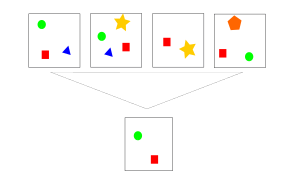
\includegraphics[width=5cm]{Bilder/rule-mining.pdf}
		\caption{Association rule-mining}
		\label{fig:abb5}
	\end{figure}